 
\documentclass[10pt, conference, compsocconf]{IEEEtran}


% *** CITATION PACKAGES ***
\usepackage{amsmath}
\usepackage{fullpage}
\usepackage[utf8]{inputenc}
\usepackage{mathtools}
\usepackage{amssymb}
\usepackage{graphicx}
\usepackage{caption}
\usepackage{subcaption}
\usepackage{amsthm}

\usepackage[usenames,dvipsnames]{color}
\usepackage[colorlinks=true,urlcolor=OliveGreen,citecolor=Blue]{hyperref}

\usepackage{soul}
\usepackage{xspace}

 

\newtheorem{theorem}{Theorem}[section]
\newtheorem{corollary}{Corollary}[theorem]
\newtheorem{lemma}[theorem]{Lemma}

\newcommand{\todo}[1]{{\color{red}\textbf{\hl{#1}}\xspace}}

%\graphicspath{{C:\Users\Manmohan\Documents\GitHub\research}}

% *** GRAPHICS RELATED PACKAGES ***
% 
\ifCLASSINFOpdf
  % \usepackage[pdftex]{graphicx}
  % declare the path(s) where your graphic files are
  % \graphicspath{{../pdf/}{../jpeg/}}
  % and their extensions so you won't have to specify these with
  % every instance of \includegraphics
  % \DeclareGraphicsExtensions{.pdf,.jpeg,.png}
\else
 
\fi

% correct bad hyphenation here
\hyphenation{op-tical net-works semi-conduc-tor}


\begin{document}

\title{Replicated Data Placement for Uncertain Scheduling}


\author{\IEEEauthorblockN{Manmohan Chaubey, Erik Saule }
\IEEEauthorblockA{Department of Computer Science\\
 University of North Carolina at Charlotte\\
 Charlotte, USA\\
 Email: mchaubey@uncc.edu, esaule@uncc.edu}
}

\maketitle


\begin{abstract}
  Scheduling theory is a common tool to analyze the
  performance of parallel and distributed computing systems, such as their load
  balance. How to distribute the input data to be able to execute a
  set of tasks in a minimum amount of time can be modeled as a
  scheduling problem. Often these models assume that the computation
  time required for each task is known accurately. However in many
  practical case, only approximate values are available at the time of
  scheduling.

  In this paper, we investigate how replicating the data required by
  the tasks can help coping with the inaccuracies of the processing
  times. In particular, we investigate the problem of scheduling
  independent tasks to optimize the makespan on a parallel system
  where the processing times of tasks are only known up to a
  multiplicative factor. The problem is decomposed in two phases: a
  first offline phase where the data of the tasks are placed and a second
  online phase where the tasks are actually scheduled.

  For this problem we investigate three different strategies, each
  allowing a different degree of replication of jobs: a) No
  Replication b) Replication everywhere and c) Replication in
  groups. We propose approximation algorithms and theoretical lower
  bound on achievable approximation ratios.  This allows us to study
  the trade-off between the number of replication and the guarantee on
  the makespan.
\end{abstract}

\begin{IEEEkeywords}
Scheduling; Uncertainty; Robustness; Replication; Approximation Algorithms; Parallel System

\end{IEEEkeywords}


\IEEEpeerreviewmaketitle

\section{Introduction}

\todo{the introduction should be structure as follow.}

\todo{one paragraph on scheduling as a tool for analyzing and
  optimizing parallel and distributed systems.Mention that in
  scheduling often processing time are known. But in practice not so
  much. Give a few references on the difficulty of predicting runtimes
  in job scheduler.}

\todo{we need a paragraph on data placement. essentially: uncertainty
  would not be a problem if the schedules could be dynamically
  changed. But in practice, the task has to run somewhere because its
  input data is there. For instance Hadoop, dooc+laf; but essentially
  in any parallel code. Even if some middleware support executing the
  task everywhere it is pays an overhead for transfering data.}

\todo{one approach for the problem is to build robust schedule. define
  robust schedule and give few quick pointers. What is better is to be
  able to arrange the schedule at runtime. What we investigate: using
  data replication to give room to the scheduler to move tasks
  around. Can it help?}

\todo{In paragraph that gives document organization. In section foo,
  we present this. In section bar we present that. This is where
  contribution should be presented. no need to give formula.}

Many real world scheduling problems related to task allocation in
parallel machines are uncertain in nature. This fact makes the class
of problem known as 'scheduling with uncertainty' or 'robust'
scheduling an important and most studied problem in
Scheduling. Robustness is the measure of to what extent an algorithm
can cope with uncertainties in a scheduling problem. Often in
scheduling problems the exact processing time of a job is not known
initially at the time of planning for job- allocation to different
machines, but they have a range outside which their values cannot
lie. The fact gives a basis to estimate the processing times and to
take job assignment decision based on these estimated values. The
actual processing time of a job can vary drastically from its
estimated one. So, any algorithm have to incur the cost of estimation
which impacts its performance negatively. A robust approach deals with
uncertainty in input parameters to minimize this cost.


The objective of our research is to study the affect on performance of
parallel machine scheduling when jobs are scheduled based on their
estimated values of processing times, and to propose scheduling
approaches that optimizes the performance in this environment. Data
placement and replication techniques can be useful in the scenario of
uncertain processing times of tasks. Effective data placement using
replication strategy allows better load balancing and hence reduces
turnaround job time. This paper is important in the sense that it
proposes different models depending upon different scenarios and
compares them based on approximation ratio and replication they
allow. Replication strategy that allows to place data in a wisely
manner offers a faster access to files required by jobs, hence
increases the job execution's performance. Replication helps in load
balancing but it have cost attached with it as it usually increases
resource usage~\cite{DBLP:journals/corr/WangJW14}. The paper deals
with this problem and chooses the scenario in which replication is
beneficial. Thus our research focus on two area of scheduling problem
i.e. task uncertainty and replication using data placement. The
scheduling problem related to data placement and task allocation is
common in heterogeneous systems and often dealt with common
approach. This paper draws qualitative analysis of the effect of
replication in data placement for uncertain scheduling with inexact
processing time of a task.

The remaining of the paper is organized as follows: we describe system
model and notations in section~\ref{sec2}. Related works are touched
in section~\ref{sec3}.  Sections~\ref{sec4}-~\ref{sec6} describes the
3 different strategies- a)No replications, b)replication is done
everywhere and c)replication is done within a group. \todo{expand per
  section}. The respective sections describe derivation of competitive
ratios for each of these strategies. Section~\ref{sec7} summarizes the
results of 3 models based on experimental results.

\section{Problem Definition}\label{sec2}
Let $J$ be a set of $n$ jobs which need to be scheduled onto a set $M$
of $m$ machines. We will use interchangeably the terms machines and
processors. Also we will use interchangeably the terms jobs and
tasks. We are considering the problems where the scheduler does not
know the processing time $p_i$ of task $i$ exactly before the task
completes.  But the scheduler has access to some estimation of the
processing time $\tilde{p_i}$ of task $i$ before making any scheduling
decisions. We assume that the actual processing time $p_i$ of a task
$i$ is within a multiplicative factor $\alpha$ of the estimated
processing time $\tilde{p_i}$. $\alpha$ is a quantity known to the
scheduler. In other words the scheduler knows that:
 \begin{equation}\label{eq1}
\frac{\tilde{p}_{i}}{\alpha}\leq p_{i}\leq \alpha \tilde{p}_{i}
\end{equation}


Assuming that the processing time of the tasks is known to be in an
interval is reasonable in many application scenarios. One could derive
bounds experimentally using machine learning techniques: for
instance~\cite{You14-ICPP} used Support Vector Machines to predict the time it
will take to run graph traversal algorithms. Models of runtime of
algorithms can also be derived analytically:
in~\cite{Erlebacher14-ICS} the authors provide bounds for the
performance of various sparse linear algebra operations using only the
size of the matrices and vector involved.

The problem is to optimize the makespan, $C_{max}$. \todo{Define
  makespan formally. Probably better if we push that at the end of the
  section.} $C_{max}^{*}$ denotes optimal makespan of a schedule $S$.

\todo{Write it so that the problem is defined in two phases, what ever
  the strategy. the strategy we follow does not change the problem.}
Depending upon a problem model the scheduling is done in two phases or
just in one phase. In Phase 1, we allocate tasks to certain processors
or group of processors depending upon a problem model.  Phase 1
chooses where data to be replicated using estimated processing time
$\tilde p_i $, for each of the task $i$. Phase 1 takes $\tilde{p_i}$,
$m$ and $\alpha$ as input and outputs set of machines, $M_j \subseteq
M $ where a task $j$ can be scheduled or is replicated.

Phase 2 takes output of phase 1 as input and \todo{write it such that
  it maps a task to a machine respecting the data allocation of phase
  1. give formal writing. Then define $E_i.$} outputs set of task
assigned to a machine $i$, $E_i \subseteq J$.  In Phase 2, we choose
\todo{avoid using we when describing problems.} actual schedule with
semi-clairvoyant algorithm which uses only approximate knowledge of
initial processing time, and after scheduling the task the actual
$p_i$ is known.  With objective to find schedule which minimizes
makespan, we investigate greedy algorithms for each of the problem
models and prove their competitive ratios. \todo{what we investigate
  has nothing to do here. This is a problem definition.}


\section{Related Work}\label{sec3}

\todo{First with $\alpha=1$ this is the classical scheduling
  problem.}\todo{NP-Hardness. cite garey johnson.} We have used
Graham's List Scheduling (LS)~\cite{Graham66} and Largest Processing
Time (LPT) algorithms~\cite{Graham69boundson} to derive approximation
ratios in different scenarios. The LS algorithm takes tasks one at a
time and assign it to the processor having least load at that time. LS
is 2-approximation algorithm and is widely used in online scheduling
problems. LPT sorts tasks in decreasing order of processing time and
assign them one at a time in this order to the processor with the
smallest current load. The LPT algorithm has worst case performance
ratio as $\frac{4}{3}-\frac{1}{3m} $ in an offline setting. Depending
upon which among these two algorithms suits more for a problem model
we have used these algorithms accordingly. \todo{PTAS from hochbaum shmoys}



Based on various models of describing uncertainty in input parameter,
uncertainty problems can be approached by various methodologies
including Reactive, stochastic, fuzzy and Robust
approach~\cite{DBLP:journals/cce/LiI08}. The bounded uncertainty model
assumes that an input parameter have value between a lower and upper
bound and is usually dealt with robust approach or sensitivity
analysis\todo{cite}. We are more interested in robust approach to deal
with uncertainty. \todo{Cut all that: ``There is very less literature
  available for scheduling with estimated processing time of a
  task. Most of the literature till now focuses on job size estimation
  with small error. Very less work is done which focuses on coping
  with less restrictive estimation for task size and which analyzes
  the effect of estimation on scheduling quantitatively''. Be factual,
  this paper takes that approach and shows that or applies it to
  that.} Wierman and Nuyens~\cite{conf/sigmetrics/WiermanN08}
introduce SMART as classification to understand size based policies
and draw analytical co-relation between response time and estimated
job size in single server problem. Dealing with uncertainty problems
with robust approach is widely used in practicality in the area of
MapReduce~\cite{Kavulya:2010:ATP:1844765.1845224}~\cite{Verma:2011:AAR:1998582.1998637},
Hadoop~\cite{Wolf:2010:FSA:2023718.2023720}~\cite{White:2009:HDG:1717298},
databases~\cite{Lipton199518} and web
servers~\cite{Cardellini99dynamicload}. HSFS and FLEX schedulers are
proposed which provides robustness in scheduling against uncertain Job
Size ~\cite{Wolf:2010:FSA:2023718.2023720} \cite{6691554}. Cannon and
Jeannot ~\cite{cj09c} provides scheduling heuristics that optimizes
both makespan and robustness in scheduling task graph on heterogeneous
system. \todo{This is not the contribution of this paper. It is mostly
  trying to understand what is the correct metric for measuring the
  robustness of a schedule. }

Most of the work on robust scheduling uses scenarios in problem
formulation to structure variability of uncertain
parameter. \todo{What does a scenario means in this context.} Daniels
and Kouvelis~\cite{citeulike:8334169} used scenarios to formulate
branch and bound based robust scheduling to cope uncertainty in
processing time of jobs in single machine. Davenport, Gefflot, and Bek
used slack based technique to add extra time to cope with
uncertainty~\cite{Davenport_slack-basedtechniques}. Gatto and Widmayer
derives bounds on competitive ratio of Graham’s online algorithm in
scenario where processing times of jobs either increase or decrease
arbitrarily due to perturbations~\cite{Gatto07}.  Their notion of
perturbed processing times is similar to our definition of estimated
processing times which can increase or decrease to actual processing
times once the jobs are processed. But unlike our work they considered
increment and decrement of job processing times as different problem
scenario. We have approached the problem with worst case scenario
where some tasks may increase and some may decrease in the same
schedule.
  
\todo{This is related works, this is not about what we do.} We have
used pro-active approach to deal with uncertainty. Through this
research we study effect of load balancing in scenario of uncertain
processing times. Based on different task assignment criteria we
propose 3 models for our problem definition, offering different degree
of task replication for load balancing. Data placement and replication
methodologies are highly used in distributed systems including
peer-to-peer and Grid systems to achieve effective data management and
improve
performance~\cite{Cirne2007213}\cite{Abawajy}\cite{4215379}. Our
notion of using replication is to increase data availability thereby
enhancing system reliability against uncertainties. With focus on
studying replication affect on performance of a schedule under
uncertainty, we have not considered cost of replication in terms of
memory utilization. Our work considers an ideal case where storage is
sufficient.  Similar work is done by Tse~\cite{DBLP:journals/tc/Tse12}
who used selective replication of documents in bi criteria problem of
minimizing load and memory in distributed file servers.


\subsection{Our Contribution}

\todo{Why do we have contribution here?}

We study the effect of load balancing through replication in classic
problem of scheduling jobs with uncertain processing times with
objective to optimize makespan. We propose 3 models based on different
degree of of replication they allow: a)No Replication i.e. $|M_j|=1
$,b) Replication is done every where i.e.$|M_j|=|M|$ and c)
Replication in groups i.e $|M_j|= m/k$ where $k$ is number of groups
each having $m/k$ processors . For each of the models we propose a two
phase algorithm based on Graham's LS and LPT; and derive performance
ratio for each. For $|M_j|=1 $, we prove that there is no algorithm
which give better performance than $\alpha^2$. Our algorithm for the
model give $\frac{2\alpha^{2}m}{2\alpha^{2}+ m-1}$ approximation. For
models with replications $|M_j|=|M|$ and $|M_j|= m/k$ the algorithms
give performance ratio of $ 1 + (\frac{m-1}{m})\frac{\alpha^{2}}{2}$
and $\frac{k\alpha^{2}}{\alpha^{2}+k-1}\left[1+ {\frac{k-1}{m}}
\right]+ {\frac{m-k}{m}}$ respectively.

\section{Strategy 1: No Replication}\label{sec4}


This section model considers the situation where the data of each task
is restricted to be on only one machine, i.e. $\forall j, |M_j|=1$.
We have a set $J$ of $ n$ jobs, and a set $M$ of $m$ machines.  Let $f
: J \mapsto M$ be a function that assigns each job to exactly one
machine. The restriction that the data of each task is deployed on a
single machine puts all the decision in phase 1: for each task,
there is only one machine is can be scheduled in phase 2.

\subsection{Lower Bound}

\todo{See how to fix numbering to remove section numbers.}
\begin{theorem}
\label{th:model1-lb}
  When $|M_j| = 1$, there is no online algorithm having competitive
  ratio better than $\frac{\alpha^{2}m }{\alpha^{2} + m-1}$.
\end{theorem}
 
\begin{proof}
  We use the adversary technique to prove the lower bound of this
  theorem. An adversary discloses the input instance piece by
  piece. He analyzes the choices made by the algorithm to change the
  part of the instance that has not been disclosed yet. That way it
  can build and instance that maximizes the competitive ratio of the
  algorithm.
 
  Let us consider an instance with $\lambda m$ tasks of equal estimated processing time
  $\forall i, \tilde{p_i} = 1$. After phase 1, let $j$ be the the most loaded
  processor which has $B$ tasks. Obviously, $B \geq \lambda$. In phase
  2 the adversary increases the processing time of the tasks on
  processor $j$ by a factor of $\alpha$ and changes the processing
  time of the other tasks by a factor of $\frac{1}{\alpha}$. So, $
  C_{max}$ = $\alpha B$ and ${C^{*}_{max}} \geq \frac{\alpha B +
    \frac{1}{\alpha } (\lambda m - B) }{m}$.  Figure \ref{fig:rara}
  depicts the online solution and the offline optimal. We have,
 \begin{equation}\nonumber
   \frac{C_{max}}{C^{*}_{max}}
   \leq \frac{\alpha^{2} B m }{\alpha^{2} B + \lambda m - B}
   =\frac{\alpha^{2}  m }{\alpha^{2}  + \frac{\lambda m}{B}  - 1}
 \end{equation}

 \todo{This proof is incorrect, we need the other inequality! We need
   a $C_{max}^* \leq something$ so that we will have $Cmax/Cmax* \geq
   somethingelse$. This should be easy to fix. Is taking the ceil of
   the expression of $Cmax$ enough?}
 
 From above expression it is clear that smaller the value of $B$, the
 smaller value of $\frac{C_{max}}{C^{*}_{max}}$. So, any algorithm
 should minimize $B$ to achieve  better performance.  For a schedule
 to be feasible the condition $B \geq \lambda$ must be
 satisfied. Irrespective of the value of $\lambda$, for $B =
 \lambda$ the value of $\frac{C_{max}}{C^{*}_{max}}$ is minimum and is
 equal to $\frac{\alpha^{2}m }{\alpha^{2} + m-1}$.

  \begin{figure}[htp]
  \centering
  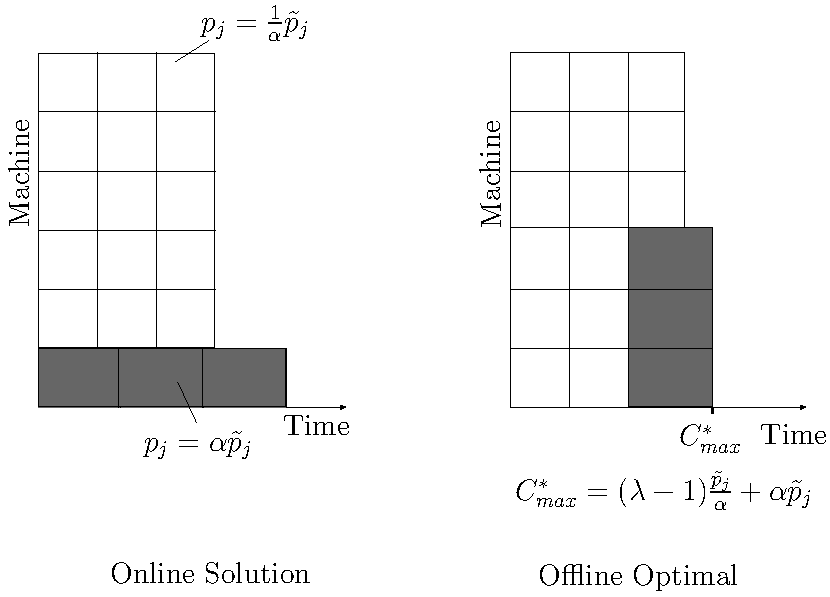
\includegraphics[width= 8 cm]{model1.pdf}
  \caption{Instance constructed by the adversary in the proof of
    theorem~\ref{th:model1-lb} with $\lambda = 3$ and $m = 6$. In the
    online solution, the adversary increased by a factor of $\alpha$
    the processing time of the task of the most loaded machine. If
    that information was available beforehand, an optimal offline
    algorithm could have distributed these longer tasks to other
    processors.  \todo{add "time" and "machine" as axis
      labels. Increase font size. Replace A and B by "online solution"
      and "Offline Optimal"}}
  \label{fig:rara}
  \end{figure}
\end{proof}    
  
  
  \begin{corollary}
  When $m$ goes to $\infty$ there is no online algorithm having competitive ratio better than $\alpha^{2}$.
  \end{corollary}
  
\subsection{Algorithm}

We introduce an algorithm, \textbf{LPT-No Choice} which is based on Graham's LPT algorithm. In phase 1, The algorithm schedules the jobs to different machines in offline mode based on non-increasing order of their estimated processing times. Just like Graham's LPT a
job is assigned to a machine having least load at that time. Adhering to the construction of the model, there is no choice of load balancing based on replication in phase 2. The performance of the algorithm depends on how much actual processing times of jobs vary from estimated ones. The actual processing time of a job may
increase or shrink significantly from its estimated value and is known exactly only after the job is processed by a machine. So, the algorithm's performance incur the cost of estimation.

\begin{theorem}
The \textbf{LPT-No Choice} has a competitive ratio of $ \frac{2\alpha^{2}m}{2\alpha^{2}+ m-1}$.
\end{theorem} 

\begin{proof}
The algorithm assigns the jobs to processors based on their estimated processing times using LPT in offline mode. So, the planned makespan considering estimated processing times of tasks, $\tilde{C}_{max}$ have following inequality relation with total estimated processing time, $\tilde{p_j}$ and estimated processing time of last task, $l$. 
\begin{equation}\label{eq2}
\tilde C_{max}\leq  \frac{\sum{\tilde p_j + (m-1) \tilde p_l} }{m}
\end{equation}

The actual makespan of a schedule, $C_{max}$, calculated after actual processing times of all the jobs are known,must be smaller than $\alpha\tilde C_{max}$. Considering this we have following inequality:
\begin{equation}\label{eq3}
 C_{max}\leq \alpha \tilde C_{max}\leq \alpha [\frac{\sum{\tilde p_j + (m-1) \tilde p_l} }{m}] 
\end{equation} 

Considering the worst case situation the processor with $\tilde C_{max}$ will see its tasks increase by $\alpha$  and the load on the  rest of the processors will by shrink  $\frac{1}{\alpha}$.  The argument behind this statement is that greater the value of ratio $\frac{C_{max}}{\sum{p_j}}$, the algorithm will give bad approximation. So increasing the load on the machine which have $C_{max} $ and deceasing the rest of the load on other processors will reach worst case scenario. So the total actual processing time is given by the  following equation.
 \begin{equation}\label{eq4}
 \sum {p_j} = \frac{\tilde p_j- \tilde C_{max}}{\alpha} + \alpha \tilde C_{max}
 \end{equation}
 
 Also the actual optimal makespan have following constraint
 \begin{equation}\nonumber 
C_{max}^{*}\geq \frac{\sum {p_j}}{m}
\end{equation}

Substituting for  $ \sum {p_j}$, we have
 \begin{equation}\nonumber 
 m C_{max}^{*}\geq \frac{\tilde p_j- \tilde C_{max}}{\alpha} + \alpha \tilde C_{max}
 \end{equation} 
\begin{equation}\nonumber 
 m C_{max}^{*}\geq \frac{\tilde p_j-[\frac{\sum{\tilde p_j + (m-1) \tilde p_l }}{m}]} {\alpha} + {C_{max}}
\end{equation}
\begin{equation}\nonumber
 m C_{max}^{*}\geq \frac{m-1}{\alpha m} [\sum \tilde p_j-\tilde p_l] + {C_{max}}
 \end{equation}

By the property of LPT $\sum \tilde p_j-\tilde p_l \geq m (\tilde C_{max}-\tilde p_l)$, putting this we have,\\
\begin{equation}\nonumber 
 m C_{max}^{*}\geq \frac{m-1}{\alpha } \left[\tilde C_{max}-\tilde p_l\right] + {C_{max}}
 \end{equation}
 
 The Graham’s LPT algorithm in normal scenario give optimal performance till two jobs are assigned to machines. But in the scenario of estimated processing times of tasks whose value can significantly vary from actual
 actual ones, any schedule using estimated values cannot guarantee optimality for even two jobs per machine. So, we consider the instance of at least two jobs per machine to derive performance ratio of our algorithm. For at least two jobs in machine having $\tilde{C}_(max)$, the processing time (estimated) of latest job, $\tilde{p_l} $ at most be equal to $\tilde{C}_(max)/2$. Putting this in the above equation, we have
\begin{equation}\nonumber
 m C_{max}^{*}\geq \frac{m-1}{\alpha } \left[\tilde C_{max}-\frac{\tilde C_{max}}{2}\right] + {C_{max}}
\end{equation}

Using equation 3,
\begin{equation}\nonumber
 m C_{max}^{*}\geq \frac{m-1}{2\alpha } \left[\frac{C_{max}} {\alpha} \right]+ {C_{max}}
\end{equation}
\begin{equation}\nonumber
 m C_{max}^{*}\geq \left[\frac{m-1}{2\alpha^{2} } +1\right]{C_{max}}
\end{equation}
\begin{equation}\nonumber
\frac{C_{max}}{C_{max}^{*}}\leq \frac{2\alpha^{2}m}{2\alpha^{2}+ m-1}
\end{equation}
\end{proof} 

\section{Model 2: replication is done everywhere}\label{sec5}

In this model, we consider putting no restriction on tasks assignment. The tasks are allowed to be replicated everywhere i.e. $\forall j, |M_{j}|=|M|$. We introduce \textbf{LPT-No Restriction }algorithm which is also a two phase algorithm. In the first phase no restriction is put into
task assignment. It is assumed that each task can be replicated on any machine. In the second phase we simply use the Longest Processing Time algorithm (LPT) using estimated processing times of tasks in non-increasing order as input.

\begin{lemma}\label{No Restriction}
 \textbf{LPT-No Restriction} has a makespan of at least $ {\frac{2}{\alpha^{2}}} p_l $ when there are at least two tasks on the machine to which the last task $l$ is scheduled. 
\end{lemma}
\begin{proof}
As there is at least one task $j$ before $l$ in the machine to which $l$ is assigned, we have
\begin{equation}\nonumber
C_{max}^{*}\geq p_l + p_j
\end{equation}	

As actual processing time of a task must be greater than $\frac{1}{\alpha}$ times of its estimated value, we have
\begin{equation}\nonumber 
C_{max}^{*} \geq \frac{1}{\alpha}\tilde p_l +  \frac{1}{\alpha} \tilde p_j 
\end{equation}

As $j$ is scheduled before $l$ using LPT on estimated values of processing times,  $\tilde p_j\geq   \tilde p_l$ holds true for tasks $l$ and $j$.  Using this, we have
\begin{equation}\nonumber
 C_{max}^{*} \geq \frac{2}{\alpha}\tilde p_l
 \end{equation}
\begin{equation}{\nonumber}
 C_{max}^{*} \geq {\frac{2}{\alpha^{2}}} p_l  \end{equation}

 \end{proof}

\begin{theorem}
\textbf{LPT-No Restriction} has a competitive  ratio of  $\frac{C_{max}}{C_{max}^{*}} \leq 1 + (\frac{m-1}{m})\frac{\alpha^{2}}{2}$
\end{theorem} 

\begin{proof}
The optimal makespan, $C_{max}^{*}$ must be at least equal to the average load on the $m$ machines. We have
\begin{equation}\label{eq7}
C_{max}^{*}\geq\frac{\sum p_j}{m}
\end{equation}

By the property of LPT the load on each machine $i$ is greater than the load on the machine which reach $C_{max}$ before the last task $l$ is scheduled. So for each machine $i$, $C_{max} \leq  \sum_{j \in E_i}^{}{p_j} + p_l$ holds true.  Summing for all the machines we have
\begin{equation}\nonumber 
mC_{max} \leq  \sum {p_j} + (m-1)p_l
\end{equation}
\begin{equation}\label{eq8}
C_{max} \leq  \frac{\sum {p_j}}{m} + \frac{(m-1)}{m}p_l
\end{equation}

Using \ref{eq7} and \ref{eq8}, we have
\begin{equation}\nonumber
\frac{C_{max}}{C_{max}^{*}} \leq 1 + {\frac{m-1}{m}}\left(\frac{p_l}{C_{max}^{*}}\right)
\end{equation}

Using Lemma \ref{No Restriction}, we have 
\begin{equation}\nonumber
\frac{C_{max}}{C_{max}^{*}} \leq 1 + \left(\frac{m-1}{m}\right)\frac{\alpha^{2}}{2}
\end{equation}

\end{proof}  

Graham's List Scheduling algorithm always has approximation of $2-\frac{1}{m}$. For $\alpha^2 < 2$, the \textbf{LPT- No Restriction} algorithm has better approximation than LS algorithm. For $\alpha^2 > 2$ the LS algorithm has better guarantee because $2p_l/\alpha^2$ becomes smaller $p_l$. As \textbf{LPT-No Restriction} is a variant of LS algorithm the optimal makespan must be at least $p_l$. So  $C_{max}^{*}\geq max[2p_l/\alpha^2,p_l]$ holds always true and hence the algorithm has approximation ratio of $max[1 + ((m-1)/2m)\alpha^{2},2-1/m ]$.   



\section{Model 3: Replication in groups}\label{sec6}
Figure \ref{fig:Model 3} shows the construction of two phases in model 3.  In this model the first phase is in offline mode and each task is pre-assigned to a particular  group of processors. In the second phase the tasks are scheduled  within the group they are assigned to in first phase.   We have a set $J$ of $ n$ tasks.  There are $k$ groups $G1$,$G2$...$Gk$.   Size of each group is equal and have $m/k$ processors within each group.  We have considered task allocation such that each task can be assigned to only one group, i.e. $\forall j$, $|M_j|= m/k$. So, this model allows each task to replicate $ m/k $ times within the group it is assigned to.

 We propose a two-phase algorithm, \textbf{LS-Group} which is based on Graham's List Scheduling algorithm. In phase 1, using LS in offline mode the algorithm pre-assign the jobs to different groups of machines. In phase 2 each task is scheduled to a particular processor within the group it was allocated in phase 1. In phase 2, the algorithm use online LS to schedule tasks to processors within each group.\\

\begin{figure*}[htp] 
\centering
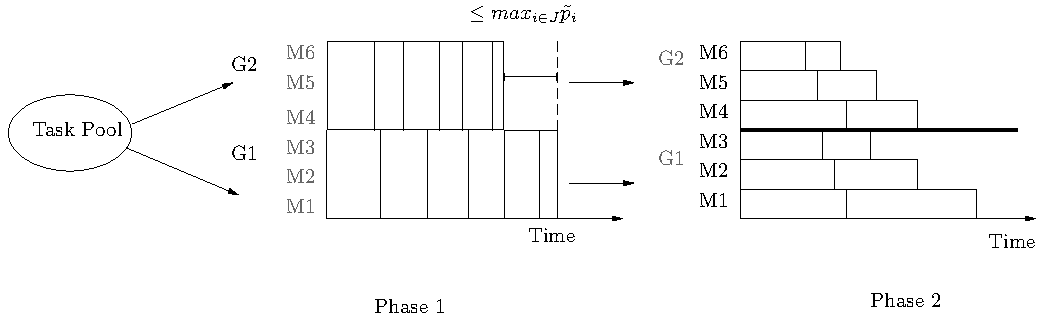
\includegraphics[width= 16 cm]{model3.pdf}
\caption{Replication in groups with $m = 6$, $k = 2$. The left figure shows tasks assignment to groups in phase 1; The right figure shows each task
assigned to a machine within a group}
\label{fig:Model 3}
\end{figure*}

\begin{theorem}
When the number of groups is $k$ the approximation ratio of \textbf{LS-Group } is $  \frac{k\alpha^{2}}{\alpha^{2}+k-1}[1+ {\frac{k-1}{m}} ]+ {\frac{m-k}{m}}   $ 
\end{theorem}
\begin{proof} 
Let us consider  that $ C_{max}$ comes from group $G1$.  As in phase 1 tasks are allocated to different groups using offline List Scheduling algorithm and taking the estimated processing times of tasks, the load difference between any two groups cannot be greater than the estimated value of largest task ${max_{i \in T}}{\tilde p_{i}}$.  So, for any group $Gl \neq G1$, We have
\begin{equation}{\nonumber}
|\sum_{i \in G1 }^{}{\tilde p_{i}}- \sum_{i \in Gl }^{}{\tilde p_{i}}| \leq {max_{i \in T}}{\tilde p_{i}}\end{equation}  \hspace*{15pt}   for all, $l = 2,3,...,k$ \\ 
Adding for all values of $l$, We have 
\begin{equation}{\nonumber}
|(k-1)\sum_{i \in G1 }^{}{\tilde p_{i}}- \sum_{l=2}^{k}\sum_{i \in Gl }^{}{\tilde p_{i}}| \leq (k-1) {max_{i \in T}}{\tilde p_{i}}
\end{equation}

\textbf{Case 1:} When $(k-1)\sum_{i \in G1 }^{}{\tilde p_{i}} > \sum_{l=2}^{k}\sum_{i \in Gl }^{}{\tilde p_{i}}$.
\begin{equation}{\nonumber}
 \sum_{l=2}^{k}\sum_{i \in Gl }^{}{\tilde p_{i}} \geq (k-1)[\sum_{i \in G1 }^{}{\tilde p_{i}}- {max_{i \in T}}{\tilde p_{i}}]
\end{equation}

As the actual processing time of tasks  can vary within a factor $\alpha$ and $\frac{1}{\alpha}$ of their estimated processing time, the following inequality holds
\begin{equation}{\nonumber}
 \alpha\sum_{l=2}^{k}\sum_{i \in Gl }^{}{{p_{i}}} \geq (k-1)[\frac{1}{\alpha}\sum_{i \in G1 }^{}{{p_{i}}}- \alpha {max_{i \in T}}{{p_{i}}}]
\end{equation}
\begin{equation}\label{eq9}
\sum_{l=2}^{k}\sum_{i \in Gl }^{}{{p_{i}}} \geq (k-1)[\frac{1}{\alpha^{2}}\sum_{i \in G1 }^{}{{p_{i}}}-  {max_{i \in T}}{{p_{i}}}]
\end{equation}

In phase 2, We are applying LS on online mode. We assume that $C_{max}$ comes from $G1$. Using LS property we can write,
\begin{equation}\label{eq10}
 C_{max} \leq \frac{\sum_{i \in G1 }^{}{{p_{i}}}}{m/k} + {\frac{m/k-1}{m/k}} p_{max}
\end{equation}

Where $p_{max}$ is actual processing time of largest task in $G1$. 

Also, $C_{max}^{*}$ must be greater than the average of the  loads on   the machines. $\sum_{i \in T }{{p_{i}}}$ represents sum of processing times all the tasks.
\begin{equation}{\nonumber}
C_{max}^{*} \geq  \frac{\sum_{i \in T }^{}{{p_{i}}}}{m}
\end{equation}

$\sum_{i \in T }{{p_{i}}}$ can be written as sum of load on $G1$ and load on rest of groups.
\begin{equation}\label{eq11}
 C_{max}^{*} \geq  \frac{\sum_{i \in G1 }^{}{{p_{i}}}+ \sum_{l=2}^{k}\sum_{i \in Gl }^{}{{p_{i}}}}{m}
\end{equation}

from \ref{eq9}, we derive
\begin{equation}{\nonumber}
 C_{max}^{*} \geq  \frac{\sum_{i \in G1 }^{}{{p_{i}}}+ (k-1)\left(\frac{1}{\alpha^{2}}\sum_{i \in G1 }^{}{{p_{i}}}-  {max_{i \in T}}{{p_{i}}}\right)}{m}
\end{equation}
\begin{equation}{\nonumber}
 m\alpha^{2}C_{max}^{*} + \alpha^{2} (k-1){max_{i \in T}}{{p_{i}}} \geq  \alpha^{2}\sum_{i \in G1 }^{}{{p_{i}}}  
\end{equation}
\begin{equation}{\nonumber}
 + (k-1)\sum_{i \in G1 }^{}{{p_{i}}} 
\end{equation}
\begin{equation}\label{eq12}
\frac{\alpha^{2}}{\alpha^{2}+k-1}\left(m C_{max}^{*}+(k-1) {max_{i \in T}}{{p_{i}}}\right) \geq \sum_{i \in G1 }^{}{{p_{i}}}  
\end{equation}

Using \ref{eq10} and \ref{eq12}, We have
\begin{equation}{\nonumber}
C_{max} \leq \frac{k\alpha^{2}}{\alpha^{2}+k-1}\left( C_{max}^{*}+\frac{(k-1)}{m} {max_{i \in T}}{{p_{i}}}\right)
\end{equation}
\begin{equation}{\nonumber}
 + {\frac{m/k-1}{m/k}} p_{max} 
\end{equation}

 As $C_{max}^{*}\geq {{max_{i \in T}}{p_{i}}}\geq p_{max}$, we have
\begin{equation}{\nonumber}
 C_{max} \leq \frac{k\alpha^{2}}{\alpha^{2}+k-1}\left( C_{max}^{*}+ {\frac{k-1}{m}}{C_{max}^{*}}\right)
  \end{equation}
 \begin{equation}{\nonumber}
   + {\frac{m-k}{m}} C_{max}^{*} 
   \end{equation}    
 
 So, for Case 1 the algorithm has approximation ratio,
 \begin{equation}{\nonumber}
\frac{C_{max}}{C_{max}^{*}} \leq \frac{k\alpha^{2}}{\alpha^{2}+k-1}\left[1+ {\frac{k-1}{m}} \right]+ {\frac{m-k}{m}} \end{equation}\\

\textbf{Case 2:} When $(k-1)\sum_{i \in G1 }^{}{\tilde p_{i}} \leq \sum_{l=2}^{k}\sum_{i \in Gl }^{}{\tilde p_{i}}$. \\

As processing times of tasks  can change within a factor $\alpha$ and $\frac{1}{\alpha}$ of their estimated values, the expression for case 2 can be written as 
\begin{equation}{\nonumber}
\sum_{l=2}^{k}\sum_{i \in Gl }^{}{ p_{i}} \geq \frac{1}{\alpha^2} (k-1)\sum_{i \in G1 }^{}{ p_{i}}
\end{equation}

Putting this value in equation \ref{eq11}, we have
\begin{equation}\label{eq13}
 C_{max}^{*} \geq \frac{\alpha^2+k-1}{m\alpha^2}\sum_{i \in G1 }^{}{ p_{i}}
\end{equation}
Using \ref{eq10} and \ref{eq13}, and as $C_{max}^{*} \geq p_{max}$, we have
\begin{equation}{\nonumber}
 C_{max} \leq \frac{k\alpha^2}{\alpha^2+k-1}C_{max}^{*}+\frac{m-k}{m}C_{max}^{*}
\end{equation}

So, for case 2 the algorithm has approximation ratio of $\frac{k\alpha^2}{\alpha^2+k-1}+\frac{m-k}{m}$.\\
Clearly, the algorithm has worst approximation for case 1.  So, the algorithm has approximation ratio of $\frac{C_{max}}{C_{max}^{*}} \leq \frac{k\alpha^{2}}{\alpha^{2}+k-1}\left[1+ {\frac{k-1}{m}} \right]+ {\frac{m-k}{m}}$



 
\end{proof}

\begin{corollary}
 When the number of groups is $2$ the approximation ratio is $ 1+ \frac{2}{1+\alpha^{2}} (\alpha^2-\frac{1}{m})  $ 
\end{corollary}

 \textbf{LS-Group} uses the LS algorithm in both its phases. A LPT-based algorithm may have better guarantee. But for no replication scenario i.e. when number of groups $k=m$, the \textbf{LS-Group} algorithm has an approximation ratio almost equal to \textbf{LPT-No choice's} when the number of machines $m$ is large and the value of $\alpha$ is within practical range. This concludes that the algorithm has a guarantee almost equal to the one of LPT-based algorithm would have for most of the practical scenario.

\section{Summary}\label{sec7}
 Table~\ref{tab:template} summarizes the results of the three algorithms in terms of approximation ratio. Based on
adversary technique, Theorem 1.1 states that there is no algorithm which can give performance better than $\alpha^2$ for the model where no replication is allowed.  LPT-No Choice is $\frac{2\alpha^{2}m}{2\alpha^{2}+ m-1}$ approximation  in this model. For the second model having $|M_j| = |M|$ (replication everywhere), LPT-No Restriction has a competitive ratio of $1 + (\frac{m-1}{m})\frac{\alpha^{2}}{2}$.  The third model having $|M_j| = m/k$, allows replication within a group of $m/k$ machines to which a task is assigned in phase 1. For this model, LS-Group algorithm has a competitive ratio of $\frac{k\alpha^{2}}{\alpha^{2}+k-1}\left[1+ {\frac{k-1}{m}} \right]+ {\frac{m-k}{m}}$ .



\begin{table*}[ht]
\centering
\begin{tabular}{|l|c|c|c|c|c|}
\hline
Replication & Approximation ratio  \\
\hline
$|M_j|=1$ & $\frac{C_{max}}{C_{max}^{*}}\leq \frac{2\alpha^{2}m}{2\alpha^{2}+ m-1}$ [Th. 1.2]  \\
 & No approximation better than $\alpha^2$ [Th. 1.1]   \\

\hline
$|M_j|=|M|$ & $\frac{C_{max}}{C_{max}^{*}} \leq 1 + (\frac{m-1}{m})\frac{\alpha^{2}}{2}$ [Th. 2.1]  \\
 & $2-\frac{1}{m}$ [Graham's LS]   \\
 \hline
 
 $|M_j|= m/k $ & $\frac{C_{max}}{C_{max}^{*}} \leq \frac{k\alpha^{2}}{\alpha^{2}+k-1}\left[1+ {\frac{k-1}{m}} \right]+ {\frac{m-k}{m}}$ [Th. 3.1]  \\
  & $\frac{C_{max}}{C_{max}^{*}} \leq  1+ \frac{2}{1+\alpha^{2}} \left(\alpha^2-\frac{1}{m}\right)$ when $k=2$ [Col. 3.1]   \\
  
  \hline
 \end{tabular}
\caption{Summary Table}
\label{tab:template}
\end{table*}


To better understand the relation between these different results we show in figure \ref{fig:Graph} how the expression of the guarantees translate to actual values in a ratio- replication space.  We picked 3 values of $\alpha$ while keeping the number of machines fixed $m=210$. For replication everywhere scenario the number of replication is full and is always equal to total number of machines.  For no replication scenario the approximation ratio is fixed for each value of $\alpha$.  For the model where replication is allowed within the group the approximation ratio decreases significantly with few replications. We observe that after a significant number of replications the ratio does not improve much further. 


\begin {figure}
\centering
\begin{subfigure}[b]{0.5\textwidth}
     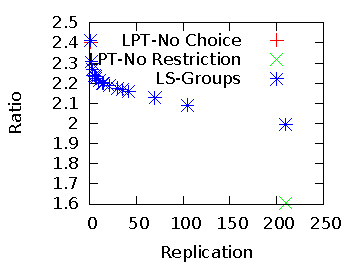
\includegraphics[width=\textwidth]{alpha_11.pdf}
     \caption{$m=210$, $\alpha=1.1$}
      \label{fig:1}
\end {subfigure} %

\begin{subfigure}[b]{0.5\textwidth}
    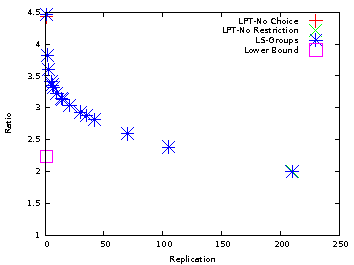
\includegraphics[width=\textwidth]{alpha_15.pdf}
     \caption{$m=210$, $\alpha=1.5$}
      \label{fig:2}
\end {subfigure} %

\begin{subfigure}[b]{0.5\textwidth}
     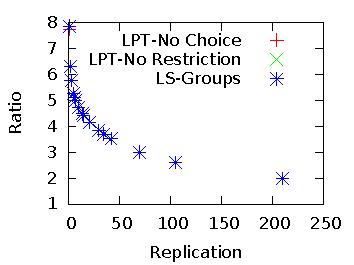
\includegraphics[width=\textwidth]{alpha_2.pdf}
     \caption{$m=210$, $\alpha=2$}
      \label{fig:3}
\end {subfigure} %


\caption{Ratio-Replication graph with m=210 and value of $\alpha$ as 1.1, 1.5 and 2}
\label{fig:Graph}
\end {figure}

\section{Conclusion and Future Work}\label{sec8}

We study the effect on performance of parallel machine scheduling when
jobs are scheduled based on their estimated values of processing
times.  We define 3 different models which uses different replication
schemes.  We propose an approximation algorithm per model and compare
their performance. We observed that even for small amount of
replications ( i.e for small group size), the guarantee of algorithm
improves drastically. So, allowing a job to be replicated over large
number of machines (large group size) might be unnecessary.

There are some open problems which can be explored as further research
work. For models allowing more than one replica of a job, there is
scope of introducing algorithms having better lower bounds.

In this research our focus was to study the effect of replication for
minimizing makespan in scheduling under uncertainty. We did not look
in the problem through memory point of view. Replication facilitates
load balancing and allows better response time by the processors and
but it is having memory cost attached with it. So, one direction to
think about the problem would be solving bi criteria problem of
optimizing load as well as memory.
 
Algorithms that replicate task without making groups of processors
could give better guarantees as there would be no restriction on the
processors where a job can be replicated. To reduce memory cost
non-constant or selective replication can be done: replicating big
tasks only could reduce the cost of replication.


\bibliographystyle{abbrv}
\bibliography{final} 



\end{document}


